\section{Human Behavior Models}
% other modeling softwares (and why they don't fit this use case)
A Human Behavior Model (HBM) attempts to model the human system’s conversion of measurable contextual information into measurable behavior outcome. 
HBMs are a set which intersects the set of computational cognitive models, both sets include approximations of cognitive processes, but in contrast with cognitive models, HBMs put a greater emphasis on the measurable in and outflows of the human system.
Cognitive models traditionally have focused on creating a comprehensible reprentation of cognitive processes, but HBMs have no such restriction and require only that a model define behavioral output as some function of contextual input.
Thus HBMs include formulations which may not be considered a cognitive model.
For instance, a model which offers little more than statistical relationship between contextual input and behavioral output may be considered an HBM.

\subsection{HBM Classes}
For our purposes, we classify HBMs into three classes based on intended application 1) Automation Agents - models developed to act as automated decision agents, 2) Emergent Behavior Studies - models developed to identify emergent behavior of a population, and 3) Cognitve HBMs - models developed for prediction and understanding of an individual's behavior.
Note that these categories are not mutually exclusive - a single HBM could theoretically fufill all three roles, but the requirements for each category are quite different, and thus existing models in each category are usually quite different.

\subsubsection{Automation Agents}
Anyone familiar with agent-based modeling is likely familiar with the behavior-desire-intent (BDI) agent architecture which has found countless applications in the automation of industry tasks such as (EXAMPLES). 
Agents of this type attempt to reproduce specific decision-making tasks reliably and predictably so that the task may be automated. 
Though extremely useful in robotics and artificial intelligence systems, these models often do not seek to represent true human-like behavior, particularly the seemingly unpredictable and irrational components. 
The goal of automation agent research is to develop an agent which can be easily told what is to be done, can express an interpretation of the given task, and can automate the task at hand reliably and accurately.

\begin{figure}[!t]
  \centering
  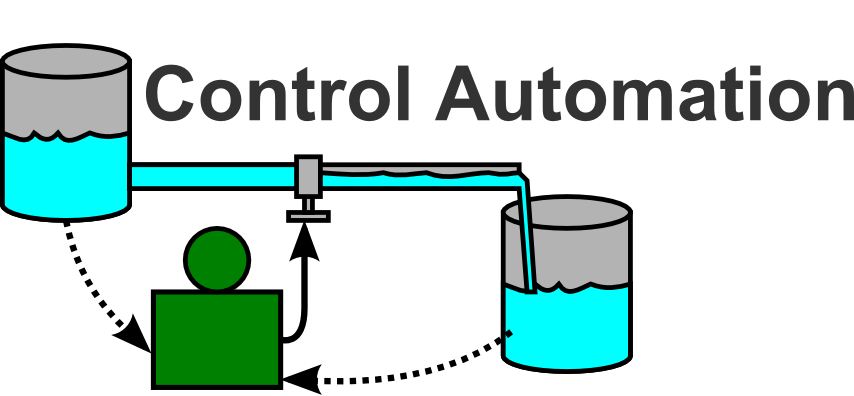
\includegraphics[width=0.5\columnwidth]{img/automationAgent}
  \caption{Human-Behavior Models designed to automate tasks such as controlling the flow of fluid between two tanks of liquid.}
  \label{automationAgent}
\end{figure}

Agents designed to replicate decision-making tasks have also found use in military strategy planning and video game AI, and through these applications have begun to incorporate variation, randomness, and ‘personality’ into the agents (\url{http://www.agent-software.com.au/applications/realistic_virtual_actors_2/}, cojack, …). 
According the terminology as defined here, this type of agent is no longer classified as an “automation agent” -- though they may be based on the BDI architecture, because the goal is no longer to simply automate a task.

\subsubsection{Emergent Behavior Studies}
Though the term agent-based modeling is often used to refer to models developed for the automation of a task or decision process (such as agents based on the BDI architecture), agent-based modeling techniques are also used to study the emergent behavior of a many-agent system. 
These emergent-behavior systems typically use a relatively simplistic agent definition and an environment with many agents to observe the behavior of the system as a whole. 
These agent models have found use in traffic simulation (Zhao 2013), MORE, and even molecular modeling (GROMACS 4.5: a high-throughput and highly parallel open source molecular simulation toolkit, Identifiability and observability analysis for experimental design in nonlinear dynamical models, bionetgen, stochsim).

\begin{figure}[!t]
  \centering
  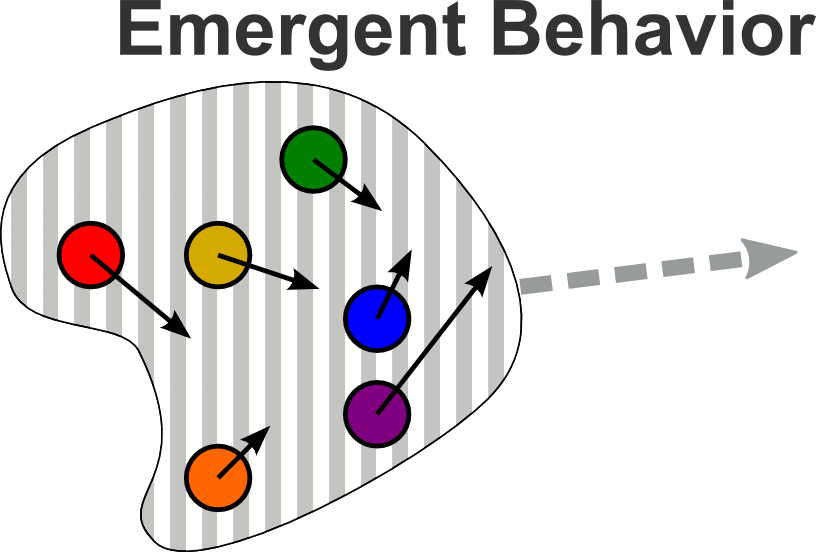
\includegraphics[width=0.5\columnwidth]{img/emergentBehavior}
  \caption{Emergent Behavior studies focus on interactions of many behavioral agents sharing one environment.}
  \label{emergentBehavior}
\end{figure}

Human behavior models developed to explore emergent behavior often neglect the intricacies of each agent’s inner workings because they are designed for efficient computation and accuracy on the level of the system rather than the individual. 

\subsubsection{Cognitive Models}
Lastly, models of human behavior are created to allow for predictive modeling of a behavioral phenomenon.
Models in this category fit the definition given by Glanz and Rimer (2005 p4): "a set of interrelated concepts, definitions and propositions that present a systematic view of events or situations by specifying relations among variables, in order to explain or predict the events or situations".
Since this type of model is useful for predicting and understanding the state of a user, formulations of theory may help overcome one of the most critical hurdles of affective computing and allow for automated intervention personalization and contextualization. 
A forecasting model can allow a human-computer interface to alter its behavior to help the user achieve a desired state. 
These models are also useful for those designing a human-computer interface or a cyber-physical system in that they can be used to estimate the ways a human may act. 

\begin{figure}[!t]
  \centering
  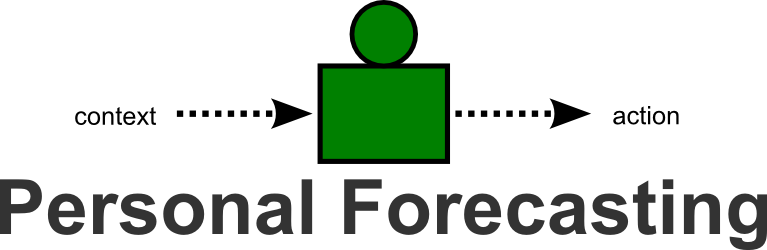
\includegraphics[width=0.5\columnwidth]{img/cognitiveHBM}
  \caption{Human behavior models which forecast human behavior focus on the translation of environmental context and internal state to future actions.}
  \label{cognitiveHBM}
\end{figure}

These models can be personalized to a subset of the population, to an individual, or may be generalizable to any healthy individual. 
Many machine learning models of human behavior and cognitive theories both fall into this category, and this type of model is of special importance to the future of automated health management systems. 
Tailored behavioral interventions, wearable sensing devices, and mHealth applications all operate based on an underlying model of human behavior which has (thus far) remained implicit in nature. 
Though all three presented classes of human behavior model may contribute to the development of the next generation of models and theories, the primary focus of this paper henceforth is on terminologies as applied to this type of human behavior model (type 3: personal forecasting).

It is important to note that behavioral forecasting models have applications outside of personalized predictions. 
Behavior forecasting models can be applied in a simulation of a population of virtual humans and compared against real data to examine the fidelity of the model or to analyze the possible effects of certain contextual stimuli. 

TODO: HBM examples /cite{Rivera}


\subsection{Existing HBM Tools}
Our review of existing tools and publications in the area of behavioral modeling has uncovered three types of tools: 1) Dynamical System Modeling Toolkits, 2) Cognitive Architectures, and 3) Agent Modeling Toolkits. 
Though each approach seeks to address the problem of human behavioral modeling, the intended use of the model is very different. 
Thus each approach makes an approximation of the human system from a different perspective, and the resulting models show little resemblence.
These three types of tools are in partial alignment with the aforementioned three classes of HBMs.

\subsubsection{Dynamical System Modeling}
Works in this group focus on generalized model-building. 
Applications include network and business analysis as well as semi-physical system modeling. 
One might be able to use these systems for modeling a human agent, but a more rigid model architecture for organizing the flow of information is needed. 
One of the contributions of the behaviorSim toolkit is the implementation of a general structure of information flow through a human agent.

Specialized modeling toolkits are often developed to create a variety of more detailed models focused around a single modeling goal. 
This is precisely the goal of the behaviorSim toolkit. 
In this search specialized toolkits focusing on neurological simulation, molecular dynamics, product inventory flow, economics, astrophysics, neurological networks, and power system modeling were all encountered in this search. 
Works on more relevant topics such as social interaction and behavioral modeling are highlighted in the spreadsheet and warrant further investigation.

\subsubsection{Cognitive Architectures}
The next group is a large set of modeling toolkits which aim to create artificial intelligence through the modeling of cognitive processes. 
Though a well implemented artificial intelligence will serve as an excellent model of human behavior, such an implementation seems far off. 
The behaviorSim toolkit takes a more empirical approach to modeling cognitive functions than existing cognitive architectures.

\subsubsection{Agent Modeling}
Agent modeling has proven useful in many industrial and commercial applications across multiple disciplines. 
Agent models are generally developed for one of two purposes: 1) to act as an intelligent actor in an automated task, or 2) to observe the emergent characteristics of many interacting agents. 
The behaviorSim toolkit does not aim to accomplish either of these goals. 
It is for this reason that the common BDI agent architecture is not suitable for modeling of human behavior based on empirical evidence. 

\section{Specialist Systems UI}
* existing work on UI for “specialist systems”
